\section{Anhang}

\subsection{Systemspezifikation}

\begin{figure}
	\centering
	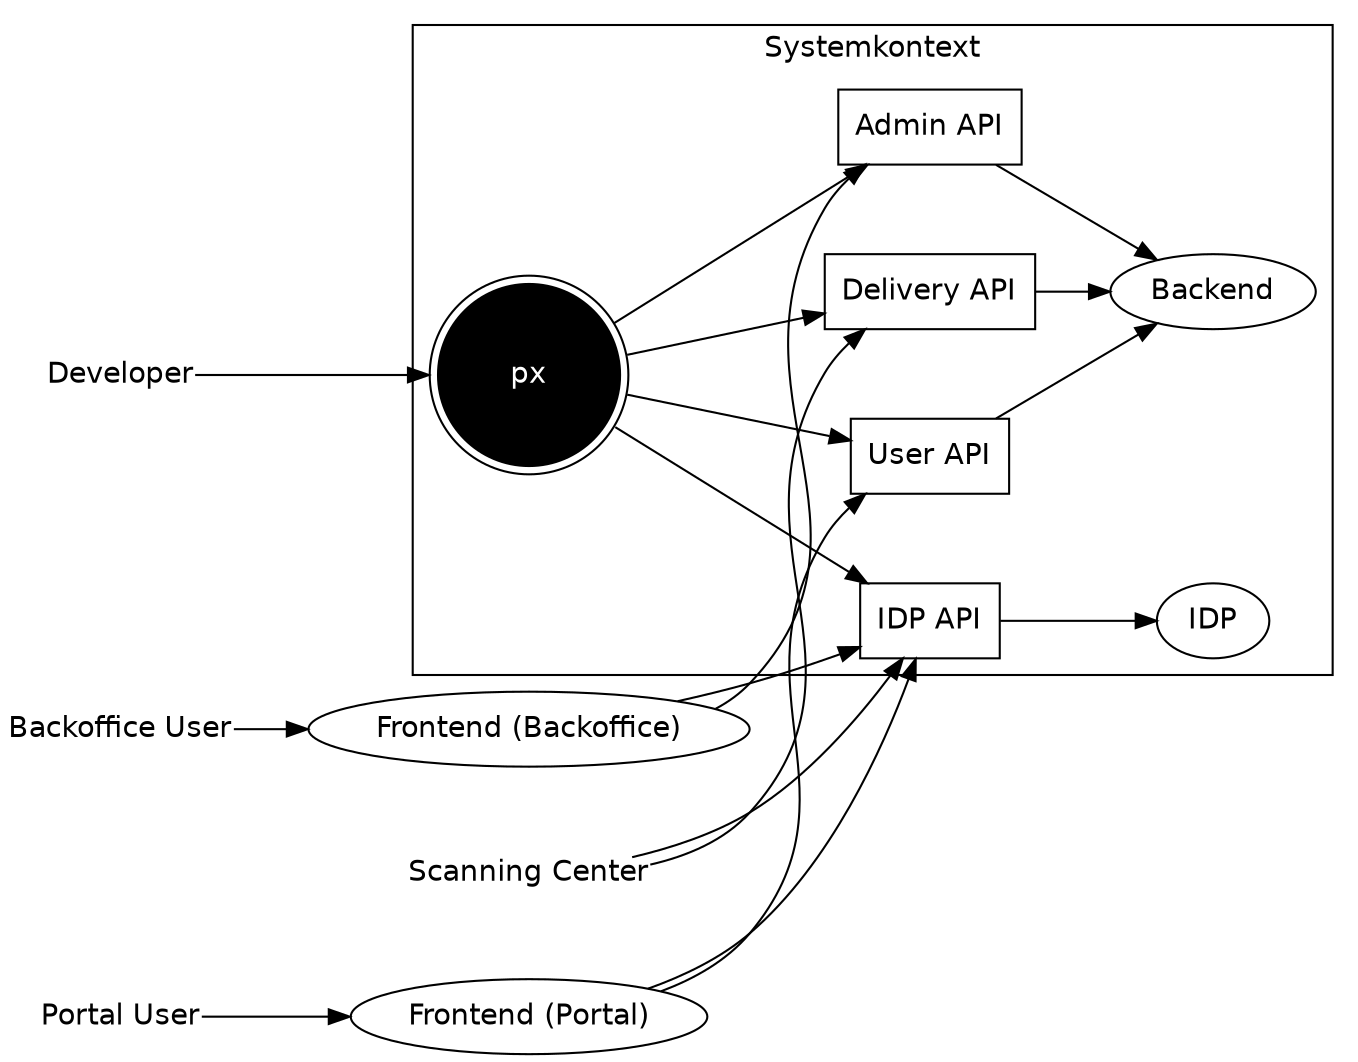
\includegraphics[width=\linewidth]{pics/kontextdiagramm.png}
	\caption{Kontextdiagramm: \texttt{px} als der Gegenstand der Arbeit innerhalb des Systemkontexts}
	\label{fig:kontextdiagramm}
\end{figure}

\subsection{Technologie-Evaluation}

- Vorgabe: PEAX API (RESTful)

\subsubsection{Programmiersprache}

Anforderungen:

\begin{description}
    \item[Installation] Die Software soll sich einfach installieren lassen.
    \item[Umgebung] Es dürfen keine besonderen Anforderungen an die Umgebung gestellt werdenm auf der \texttt{px} läuft.
    \item[Plattformen] Die Software soll auf allen gängigen Betriebssystemen (Windows, mac OS, Linux) lauffähig sein.
    \item[Einheitlichkeit] Der Client soll überall die gleiche Befehlssyntax haben.
    \item[Performance] Ein Command Line Client soll in Skripten verwendet werden können, wodurch das Programm sehr oft in kurzem Zeitraum aufgestartet werden muss.
\end{description}

Java erfordert die lokale Installation einer JRE in der richtigen Version. Ausserdem werden Wrapper-Skripts benötigt (\texttt{java -jar px.jar} ist nicht praktikabel).

Python, Ruby, Perl und andere Skriptsprachen benötigen ebenfalls einen vorinstallierten Interpreter in der richtigen Version.

Zwar gibt es mit Mono eine Variante von .Net, die überall lauffähig ist, hier werden aber wiederum eine Laufzeitumgebung bzw. vorinstallierte Libraries benötigt.

Am besten geeignet sind kompilierte Sprachen (C, C++, Go, Rust, Nim). Mit einer statischen Kompilierung lässt sich das ganze Programm in eine einzige Binärdatei überführen, welches denkbar einfach zu installieren ist (Kopieren nach einem der Verzeichnisse innerhalb von \texttt{\$PATH}).

Für JavaScript gibt es mit QuickJS seit kurzem die Möglichkeit, JavaScript zu Binärdateien zu kompilieren. Dies funktioniert aber nicht auf allen Plattformen, ausserdem ist QuickJS noch experminentell und noch nicht für den produktiven Einsatz geeignet.

In die engere Auswahl kommen Go und Rust, da der Autor dieser Arbeit mit diesen Programmiersprachen bereits Erfahrungen im Studium machen konnte. (Mit C++ noch keine Erfahrungen gemacht. Mit C Erfahrungen gemacht, wodurch es als sehr aufwändig erscheint, einen HTTP-Client zu schreiben.)

\subsubsection{Go}

\begin{itemize}
    \item einfach zu lernen (wenige Keywords und Features), dafür keine Features wie Generics und map/filter/reduce
    \item gutes und übersichtliches Tooling
    \item Cross-Compilation ohne Zusatztools möglich
    \item Kompilierung zu statischen Binaries, die jedoch recht gross ausfallen (Prototyp: ca. 4 MB)
    \item Kompilierung extrem schnell
    \item umfassende und qualitativ hochwertige Standard Library, inkl. HTTP-Library
    \item persönlich bereits viel damit gearbeitet, positive Erfahrungen damit gemacht
    \item Error Handling aufwändig, führt aber zu sehr solidem, wenn auch repetitivem Code
    \item vergleichbare Software (\texttt{oc}: OpenShift Command Line Client, \texttt{docker}: Docker Command Line Client) ist ebenfalls in Go geschrieben und bei uns täglich erfolgreich im Einsatz
    \item fügt sich sehr gut in UNIX-Philosophie ein (Tooling, Libraries)
    \item Einfaches Interface für nebenläufige Programmierung (Goroutines und Channels)
    \item Performance im Bereich von Java, jedoch tieferer Memory-Footprint
\end{itemize}

\subsection{Rust}

\begin{itemize}
    \item viele Features, dafür aber schwer zu lernen (Lifetimes, Borrowing, siehe PCP)
    \item gutes und übersichtliches Tooling
    \item Kompilierung in statische Binaries, die relativ schlank ausfallen
    \item Kompilierung eher langsam
    \item Cross-Compilation benötigt Zusatztools
    \item wenig Erfahrung damit gesammelt
    \item Standard Library bewusst schlank gehalten, dafür viele externe Libraries benötigt
    \item extrem ausdrucksstarke Sprache mit starkem Typsystem
    \item diverse Rust-Utils erfolgreich persönlich im Einsatz (rg, bat, hexyl, battop)
    \item erstklassige Performance (im Bereich von C/C++)
\end{itemize}

\subsection{Libraries}
